\chapter{सूक्ष्मजीव और संक्रमण}\label{ch:g9:microbes-and-infection}

पहली कक्षा के अनदेखे \omterm{def:g1:healthy-habits:germs}{रोगाणुओं} (\cref{def:g1:healthy-habits:germs}) से ही
वे इस किताब के साथ-साथ चले हैं: नानबाई-ख़ाने में मज़दूरी तक चढ़े
(\cref{ch:g6:producing-our-food}), \omterm{def:g6:decomposers-and-soil:soil}{मिट्टी} में \omterm{def:g6:decomposers-and-soil:decomposers}{अपघटक} टोलियों तक, और
अस्पताल के वार्ड में विकसित होते दुश्मन तक
(\cref{ex:g9:how-species-change:resistance})। यह अध्याय आख़िरकार
सूक्ष्मजीवों का पूरा लेखा देता है: वे हैं क्या, वह नुक़सान करने वाली
अल्पसंख्या हमला कैसे करती है, और शरीर की बाहरी हिफ़ाज़तें --- तथा हमारी
अपनी --- दरवाज़े कैसे थामे रखती हैं।

\section{सूक्ष्मजीवों की दुनिया}

\begin{definition}[सूक्ष्मजीव, छँटे हुए]\label{def:g9:microbes-and-infection:sorted}
\emph{सूक्ष्मजीव}\index{सूक्ष्मजीव} वे \omterm{def:g6:exploring-our-environment:components}{सजीव} हैं जो बिना किसी मदद के
देखे जाने लायक़ नहीं होते। उनके मुख्य प्रकार:
\begin{itemize}
  \item \emph{जीवाणु}\index{जीवाणु}: बिना असली \omterm{def:g6:cell-unit-of-life:parts}{केंद्रक} वाली अकेली
        \omterm{def:g5:first-look-at-cells:cell}{कोशिकाएँ}, तुम्हारी \omterm{def:g5:first-look-at-cells:cell}{कोशिकाओं} से कहीं छोटी, और तेज़ी से बँटती
        हुईं (\cref{def:g6:cell-unit-of-life:unicellular} वाली दुनिया)
        --- हर जगह, और गिनती से बाहर तादाद में;
  \item \emph{\omterm{def:g6:cell-unit-of-life:unicellular}{एककोशिकीय} \omterm{def:g6:decomposers-and-soil:decomposers}{कवक} और बाक़ी}: ख़मीर
        (\cref{ex:g6:producing-our-food:bread}), फफूँदों के \omterm{def:g4:plants-without-seeds:spore}{बीजाणु}, और
        तालाब की बूँद के तैराक;
  \item \emph{विषाणु}\index{विषाणु}: उनसे भी छोटे, और क़िस्म में ही
        अलग --- यानी आनुवंशिक इबारत का एक बँधा हुआ टुकड़ा
        (\cref{def:g9:genes-and-dna:dna} वाले अक्षर) एक ग़िलाफ़ में,
        और \emph{न कोई \omterm{def:g5:first-look-at-cells:cell}{कोशिका}, न अपना कोई जीवन}: कोई विषाणु तब तक कुछ
        नहीं करता जब तक वह किसी जीवित \omterm{def:g5:first-look-at-cells:cell}{कोशिका} में घुसकर उस \omterm{def:g5:first-look-at-cells:cell}{कोशिका} की
        पढ़ने वाली मशीनरी को घुसपैठिए की इबारत की नक़ल पर न लगा दे।
        \cref{prop:g1:living-or-not:signs} की निशानियों पर विषाणु
        जीवन के बिलकुल किनारे बैठते हैं।
\end{itemize}
\end{definition}

\begin{proposition}[ज़्यादातर बेज़रर, और अक्सर ज़रूरी]\label{prop:g9:microbes-and-infection:mostly}
नुक़सान वाली शोहरत दरअसल अल्पसंख्या की रपट है। ज़्यादातर \omterm{def:g9:microbes-and-infection:sorted}{सूक्ष्मजीव}
हमारी परवाह ही नहीं करते; और बहुत-से हमारी सेवा करते हैं: \omterm{def:g6:decomposers-and-soil:decomposers}{अपघटक} टोलियाँ
(\cref{def:g6:decomposers-and-soil:decomposers}), भोजन बनाने वाले
मज़दूर, \omterm{def:g6:decomposers-and-soil:soil}{मिट्टी} के रसायनकर्मी --- और ख़ुद तुम्हारे \emph{बसे हुए
सूक्ष्मजीव}\index{बसे हुए सूक्ष्मजीव}: यानी वे खरबों बेज़रर \omterm{def:g9:microbes-and-infection:sorted}{जीवाणु}, जो
\omterm{def:g1:the-five-senses:sense}{त्वचा} और आँत पर क़ालीन बिछाए हैं, \omterm{def:g4:journey-of-food:digestion}{पाचन} में मदद करते हैं, और सिर्फ़ जगह
घेरकर घुसपैठियों को उतरने ही नहीं देते। बीमारी सिर्फ़ एक छोटी
अल्पसंख्या --- यानी \emph{रोगजनक}\index{रोगजनक} --- फैलाते हैं।
\end{proposition}
\admitted

\begin{example}[एक शरीर, तीन रिश्ते]\label{ex:g9:microbes-and-infection:relations}
इस वक़्त तुम्हारी \omterm{def:g1:the-five-senses:sense}{त्वचा} पर: अरबों की तादाद में बसे हुए, वह सतह थामे हुए
(पहला रिश्ता: गठबंधन)। नाश्ते में तुम्हारे दही में: मज़दूर, हुक्म पर
खट्टा करते हुए (दूसरा रिश्ता: नौकरी,
\cref{ex:g6:producing-our-food:yogurt})। और कोठरी में पड़ी उस ज़ंग लगी
कील पर: टिटनेस के \omterm{def:g9:microbes-and-infection:sorted}{जीवाणु} के \omterm{def:g4:plants-without-seeds:spore}{बीजाणु}, किसी गहरे कटाव के इंतज़ार में (तीसरा
रिश्ता: वही \omterm{prop:g9:microbes-and-infection:mostly}{रोगजनक} अल्पसंख्या, और \cref{ch:g9:immune-defenses} तथा
टिटनेस के टीके की वजह)।
\end{example}

\section{संक्रमण: हमला, चरणों में}

\begin{definition}[संक्रमण के चरण]\label{def:g9:microbes-and-infection:stages}
\emph{संक्रमण}\index{संक्रमण} चरणों में चलता है, और हर चरण का अपना नाम
है:
\begin{enumerate}
  \item \emph{संचरण}: \omterm{prop:g9:microbes-and-infection:mostly}{रोगजनक} सफ़र करता है --- छुई हुई सतहें और हाथ,
        खाँसी की बूँदें, दूषित भोजन तथा पानी, \omterm{prop:g4:journey-of-food:absorb}{रक्त}, और वह सहवास वाला
        रास्ता भी जिसका ज़िक्र \cref{def:g8:contraception:condom} ने
        किया था;
  \item \emph{प्रवेश}: किसी दरार से --- कटी हुई \omterm{def:g1:the-five-senses:sense}{त्वचा}, या शरीर के खुले
        दरवाज़े: हवा-मार्ग, आँत, और ऊपर वाले रास्ते;
  \item \emph{बढ़त}: गरम, गीले और खिलाए हुए में, आए हुए बँटने लगते हैं
        --- \omterm{def:g9:microbes-and-infection:sorted}{जीवाणु} \cref{prop:g6:decomposers-and-soil:speed} वाले
        परिस्थिति-नियम से, और घंटों में अपनी तादाद दोगुनी करते हुए; और
        \omterm{def:g9:microbes-and-infection:sorted}{विषाणु} \omterm{def:g5:first-look-at-cells:cell}{कोशिकाओं} को नक़ल-ख़ाना बनाकर;
  \item \emph{बीमारी}: \omterm{def:g9:heredity-and-traits:traits}{लक्षण} --- ख़ुद उस नुक़सान से, \omterm{def:g9:microbes-and-infection:sorted}{जीवाणुओं} के
        ज़हरों से, और कुछ हद तक (अगला अध्याय) ख़ुद हिफ़ाज़त की लड़ाई
        से।
\end{enumerate}
\end{definition}

\begin{example}[दो हमलावर, आमने-सामने]\label{ex:g9:microbes-and-infection:contrast}
कटाव का \omterm{def:g9:microbes-and-infection:sorted}{जीवाणु} बनाम सर्दी का ज़ुकाम वाला \omterm{def:g9:microbes-and-infection:sorted}{विषाणु}। \omterm{def:g9:microbes-and-infection:sorted}{जीवाणु}: दरार से घुसता
है, गरम गीले ऊतक में \omterm{def:g5:first-look-at-cells:cell}{कोशिकाओं} के \emph{बीच} बढ़ता है, और उसका कचरा
आस-पड़ोस को ज़हरीला कर देता है --- यानी पके हुए उँगली के घाव की टीस और
पीप। \omterm{def:g9:microbes-and-infection:sorted}{विषाणु}: किसी बूँद पर सवार होकर हवा-मार्ग की परत तक पहुँचता है, ख़ुद
उन परत वाली \omterm{def:g5:first-look-at-cells:cell}{कोशिकाओं} में घुसता है, और हर हड़पी हुई \omterm{def:g5:first-look-at-cells:cell}{कोशिका} नाकाम होने से
पहले नक़लों की एक भीड़ छोड़ जाती है --- यानी उसके रास्ते का कच्चा गला और
बहती नाक। कार्य-प्रणालियाँ अलग; और जो प्रतिजैविक पहले को भूखा मारता है वह
दूसरे को छू तक नहीं सकता, क्योंकि दूसरा तो \emph{तुम्हारी} ही मशीनरी
उधार लेता है, और उस पर निशाना साधने वाली दवाएँ बनाना मुश्किल है।
\end{example}

\section{दरवाज़े थामना}

\begin{proposition}[पहली हिफ़ाज़तें]\label{prop:g9:microbes-and-infection:doors}
किसी भी लड़ाई से पहले शरीर अपनी सरहदें थामे रखता है:
\begin{itemize}
  \item \emph{\omterm{def:g1:the-five-senses:sense}{त्वचा}}: सूखी, परतदार, और ख़ुद को नया करती हुई --- यानी
        वह दीवार (\cref{def:g1:the-five-senses:sense} वाला अंग,
        पहरे पर);
  \item \emph{परतें और उनकी बुहारियाँ}: हवा-मार्गों की सफ़ाई करती सतहें
        (\cref{prop:g7:lungs-and-gas-exchange:smoke} ने उन्हें लदा हुआ
        दिखाया था), आँसुओं तथा \omterm{def:g4:journey-of-food:tract}{लार} का धोता हुआ रसायन, और \omterm{def:g4:journey-of-food:tract}{आमाशय} का
        अम्ल-स्नान (\cref{pb:g7:digestion-and-nutrients:1} पचाते-पचाते
        बाँझ भी कर देता है);
  \item \emph{बसे हुए}: उनकी घेरी हुई ज़मीन, जहाँ उतरने की जगह ही
        कम है;
\end{itemize}
और \omterm{def:g1:healthy-habits:hygiene}{स्वच्छता} उन्हें और आगे बढ़ा देती है: \cref{met:g1:healthy-habits:hands}
वाला साबुन (अब अपनी पूरी कार्य-प्रणाली के साथ --- यानी संचरण तोड़ा हुआ),
सुरक्षित पानी, पकाया हुआ तथा ठंडा रखा भोजन
(\cref{rem:g6:producing-our-food:goodbad} वाला \omterm{def:g6:exploring-our-environment:conditions}{परिस्थितियों} से इनकार),
बाँझ की हुई सुई, और \omterm{def:g8:contraception:condom}{कंडोम} की रोक। इस किताब का \omterm{def:g1:healthy-habits:hygiene}{स्वच्छता} का हर नियम कोई एक
संचरण या प्रवेश का चरण है, रोका हुआ।
\end{proposition}
\admitted

\begin{omfigure}
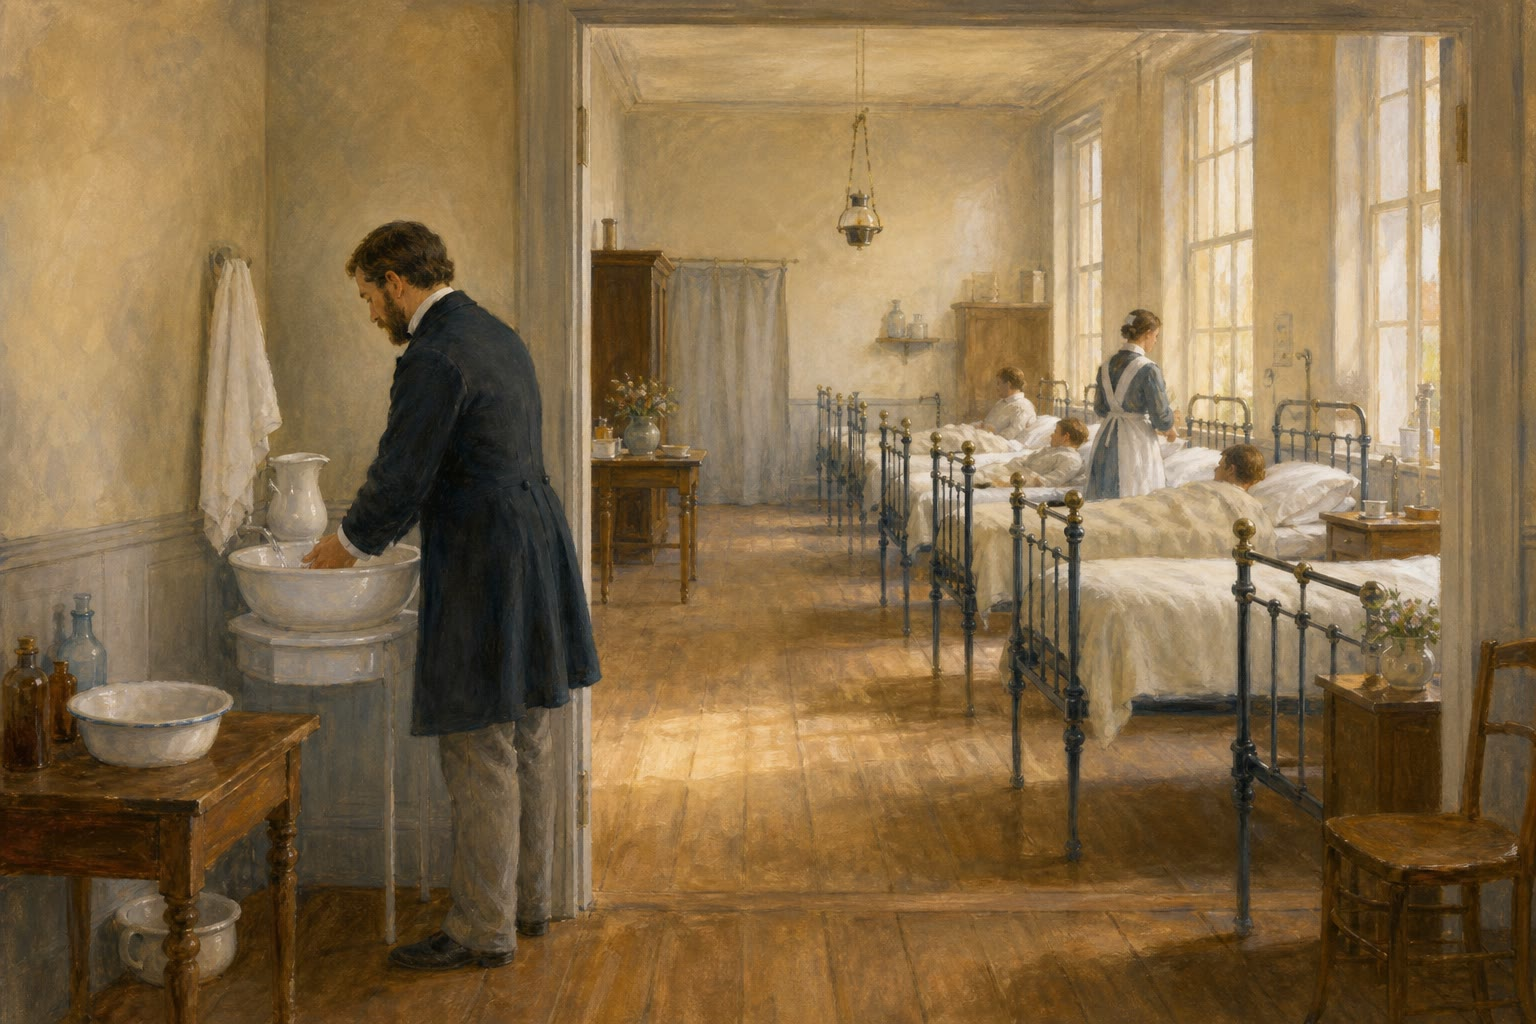
\includegraphics[width=0.6\linewidth]{images/book1/ai/g9-microbe-washing.jpg}

{\small इतिहास की सबसे सस्ती दवा: वार्ड के दरवाज़े पर रखा एक तसला, जो उन
हरकारों को रोक देता है जिन्हें कोई \omterm{def:g1:the-five-senses:sense}{आँख} नहीं देख सकती।}
\end{omfigure}

\begin{example}[वे दो डॉक्टर जिन्होंने आँकड़े बदल दिए]\label{ex:g9:microbes-and-infection:history}
इतिहास दो नामों पर टिका है। ज़ेमेलवाइस, 1840 के दशक का वियना: जब डॉक्टर
शव-परीक्षा के कमरे और प्रसव-कक्ष के बीच हाथ धोने लगे तो उनके प्रसूति
वार्ड में प्रसव-ज्वर से होने वाली मौतें ढह गईं --- यानी संचरण उससे भी
पहले तोड़ा गया, जब किसी ने उस मुसाफ़िर को देखा तक नहीं था। और पास्तूर ने,
एक पीढ़ी बाद, ख़ुद उन मुसाफ़िरों को दिखा दिया: शराब को खट्टा करते,
रेशम-कीड़ों को मारते और घावों को संक्रमित करते वे ``बुरी हवा'' नहीं,
\omterm{def:g9:microbes-and-infection:sorted}{सूक्ष्मजीव} थे --- और गरमी (उनका \emph{पास्तुरीकरण}) या बाँझ करना उन्हें
रोक देता था। रोगाणु-सिद्धांत ने एक ही ज़िंदगी के भीतर अस्पतालों को
ख़तरों से हिफ़ाज़तों में बदल दिया।
\end{example}

\begin{omfigure}
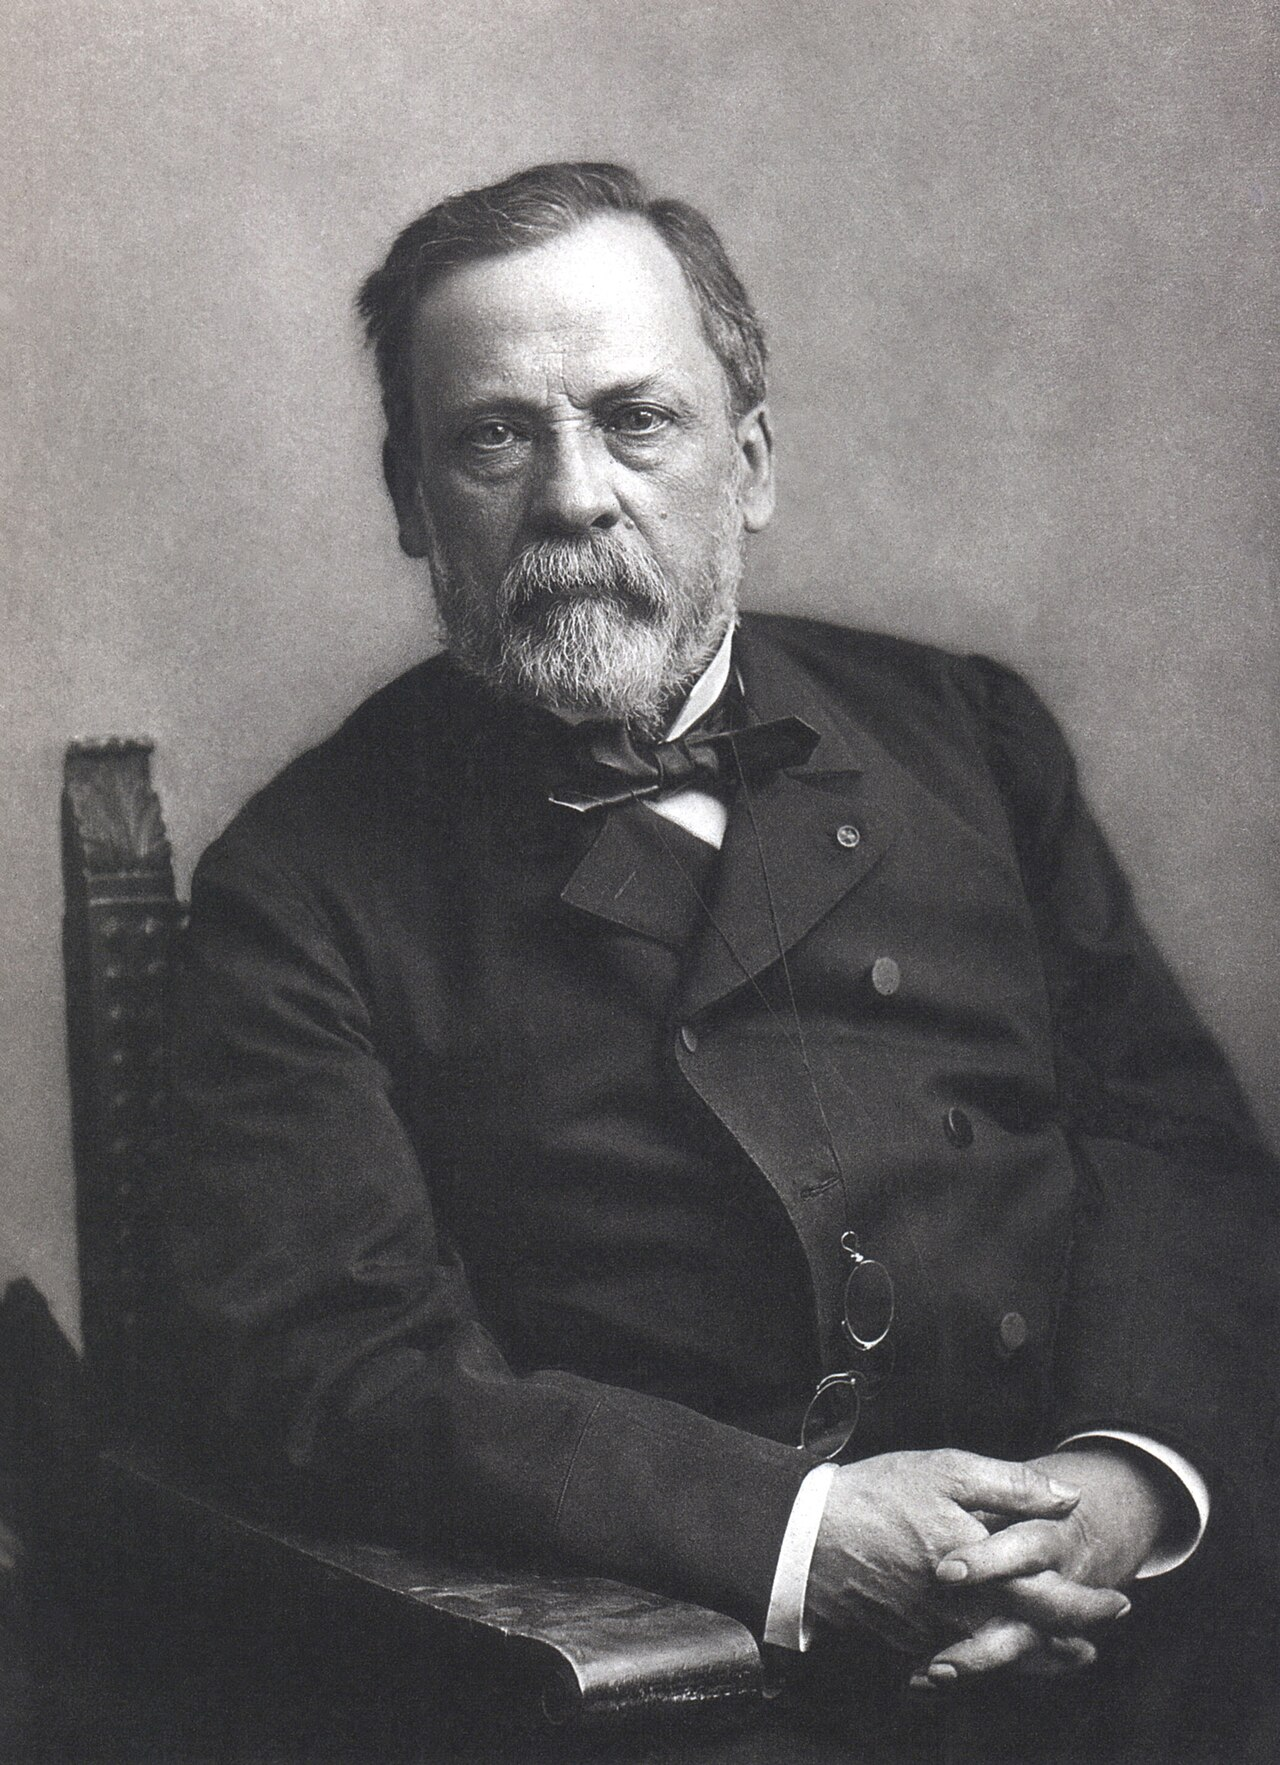
\includegraphics[width=0.42\linewidth]{images/book1/pasteur.jpg}

{\small लुई पास्तूर, पॉल नादार की खींची तस्वीर में: वही वैज्ञानिक,
जिन्होंने उन अनदेखे मुसाफ़िरों को ख़ुद दिखा दिया।}
\end{omfigure}

\begin{method}[संक्रमण के ख़तरे की जाँच]\label{met:g9:microbes-and-infection:audit}
किसी भी हालत के लिए --- रसोई, घाव, वार्ड, भीड़:
\begin{enumerate}
  \item मुमकिन \omterm{prop:g9:microbes-and-infection:mostly}{रोगजनक} और उसकी क़िस्म का नाम बताओ (\omterm{def:g9:microbes-and-infection:sorted}{जीवाणु}, \omterm{def:g9:microbes-and-infection:sorted}{विषाणु},
        \omterm{def:g6:decomposers-and-soil:decomposers}{कवक});
  \item तुम तक उसके संचरण के रास्ते का पीछा करो;
  \item उसके प्रवेश का दरवाज़ा ढूँढ़ो;
  \item पूछो कि उसे बढ़ाता क्या है --- गरमाहट, नमी, भोजन, समय;
  \item और सबसे सस्ता चरण रोको: धोओ, पकाओ, ढको, ठंडा रखो, बाँझ करो,
        टीका लगवाओ (\cref{ch:g9:immune-defenses} आख़िरी वाला समझाता
        है)।
\end{enumerate}
\end{method}

\section{अभ्यास}

\begin{exercise}[$\star$]\label{exo:g9:microbes-and-infection:1}
सूक्ष्मजीवों के मुख्य प्रकार बताओ, और यह भी कि \omterm{def:g9:microbes-and-infection:sorted}{विषाणुओं} को अलग क्या करता
है।
\end{exercise}

\begin{exercise}[$\star$]\label{exo:g9:microbes-and-infection:2}
\omterm{prop:g9:microbes-and-infection:mostly}{बसे हुए सूक्ष्मजीव} क्या हैं, और वे कौन-सी दो सेवाएँ देते हैं?
\end{exercise}

\begin{exercise}[$\star$]\label{exo:g9:microbes-and-infection:3}
\omterm{def:g9:microbes-and-infection:stages}{संक्रमण} के चारों चरण गिनाओ, और हर एक का एक-एक उदाहरण भी।
\end{exercise}

\begin{exercise}[$\star$]\label{exo:g9:microbes-and-infection:4}
पके हुए कटाव और ज़ुकाम की तुलना करो: हर हमलावर बढ़ता कहाँ है?
\end{exercise}

\begin{exercise}[$\star$]\label{exo:g9:microbes-and-infection:5}
पहली हिफ़ाज़तों में से चार बताओ, और यह भी कि हर एक कौन-सा चरण थामती है।
\end{exercise}

\begin{exercise}[$\star$]\label{exo:g9:microbes-and-infection:6}
ज़ेमेलवाइस के हाथ धोने ने क्या तोड़ा, और पास्तूर ने उसमें क्या जोड़ा?
\end{exercise}

\begin{exercise}[$\star\star$]\label{exo:g9:microbes-and-infection:7}
प्रतिजैविक ज़ुकाम को अनछुआ क्यों छोड़ देते हैं? जवाब दोनों हमलावरों की
कार्य-प्रणालियों से दो।
\end{exercise}

\begin{exercise}[$\star\star$]\label{exo:g9:microbes-and-infection:8}
बचपन के तीन स्वच्छता-नियमों (\cref{ch:g1:healthy-habits}) को चरण-रोक की
तरह दोबारा निकालो, और कार्य-प्रणाली का नाम भी लो।
\end{exercise}

\begin{exercise}[$\star\star$]\label{exo:g9:microbes-and-infection:9}
\cref{met:g9:microbes-and-infection:audit} को किसी गर्मी की सैर वाले उस
मुर्ग़-सलाद पर चलाओ, जो तीन घंटे गाड़ी में गरम होता रहा।
\end{exercise}

\begin{exercise}[$\star\star$]\label{exo:g9:microbes-and-infection:10}
हाथ बार-बार धोने से ज़्यादा \emph{कामों के बीच} धोना क्यों मायने रखता
है? (जवाब ज़ेमेलवाइस के वार्ड में है।)
\end{exercise}

\begin{exercise}[$\star\star$]\label{exo:g9:microbes-and-infection:11}
\cref{ex:g9:how-species-change:resistance} वाले वार्ड को इस अध्याय में
रखो: वह प्रतिजैविक किस चरण पर हमला करता है, और उसका अधूरा इस्तेमाल क्या
पाल देता है?
\end{exercise}

\begin{exercise}[$\star\star\star$]\label{exo:g9:microbes-and-infection:12}
``कोई \omterm{def:g9:microbes-and-infection:sorted}{विषाणु} ऐसी इबारत है जो कोई छापाख़ाना उधार ले लेती है।'' इस तस्वीर
को \cref{def:g9:genes-and-dna:dna} और
\cref{def:g9:microbes-and-infection:sorted} से खोलो --- और उसी से बताओ
कि \omterm{def:g9:microbes-and-infection:sorted}{विषाणु} जीवन के किनारे पर क्यों बैठते हैं, और उन पर दवा का निशाना साधना
मुश्किल क्यों है।
\end{exercise}

\section{समस्या: फैलाव की नोटबुक}

\begin{problem}[{सप्ताहांत समस्या --- स्कूल में एक फैलाव,
चरण-दर-चरण पीछा किया हुआ}]\label{pb:g9:microbes-and-infection:1}
एक (काल्पनिक) स्कूली फैलाव: एक ही हफ़्ते में कक्षा 9ख के आधे बच्चे बुख़ार
और खाँसी की ख़बर देते हैं; और फिर बाक़ी कक्षाओं में भी मामले छिटकने लगते
हैं। स्कूल की नर्स फैलाव की एक नोटबुक रखती है और जीव विज्ञान की कक्षा से
उसे पढ़ने में मदद माँगती है।

\medskip\noindent\textbf{भाग I --- फैलाव पढ़ना।}
\begin{enumerate}
  \item पहला मामला --- यानी सूचकांक --- कक्षा 9ख में बैठता था; और अगले
        आठ उसी की क़तार तथा उसके टेबल-टेनिस के साथियों के हैं। संचरण का
        मुमकिन रास्ता बताओ, और प्रवेश का दरवाज़ा भी।
  \item शुरू में मामले हर दो दिन में दोगुने होते हैं। यह किस चरण का
        गणित दिखा रहा है, और अगर वह कारक कोई \omterm{def:g9:microbes-and-infection:sorted}{विषाणु} है तो नक़ल किसकी
        मशीनरी कर रही है?
  \item नर्स की जाँच-सूची: बुख़ार का चढ़ना, खाँसी, कच्चा गला। ये \omterm{def:g9:heredity-and-traits:traits}{लक्षण}
        कौन-सा चरण बताते हैं, और वे किन दो स्रोतों से उठते हैं?
  \item यह फैलाव ठीक उसी हफ़्ते की दोनों पूरे-स्कूल वाली सभाओं पर
        कक्षाएँ लाँघ क्यों गया?
\end{enumerate}

\medskip\noindent\textbf{भाग II --- जवाबी हमला।}
\begin{enumerate}[resume]
  \item स्कूल के उपाय: बीमार विद्यार्थी घर; खिड़कियाँ खुलीं
        (\cref{exo:g4:breathing:10}); हाथ धोने की मश्क़; और साझा
        सामान पोंछा हुआ। हर उपाय को उसका रोका हुआ चरण सौंपो।
  \item एक अभिभावक सबके लिए प्रतिजैविक की माँग करते हैं। \omterm{def:g9:microbes-and-infection:sorted}{विषाणु} वाले
        फैलाव के लिए डॉक्टर का जवाब लिखो --- और वह चयन वाली चेतावनी भी
        (\cref{exo:g9:how-species-change:10}), अगर प्रतिजैविक फिर भी
        बिखेर दिए जाएँ।
  \item ठीक उसी वक़्त भोजनालय बिना फ़्रिज रखी एक मिठाई से जुड़े पेट के
        दो मामलों की ख़बर देता है। उस बग़ली फैलाव की जाँच
        \cref{met:g9:microbes-and-infection:audit} से करो --- अलग
        क़िस्म का कारक, अलग चरण।
  \item नर्स मामलों को बेतरतीब मानकर चलने के बजाय यह नक़्शा क्यों
        बनाती है कि \emph{कौन कहाँ बैठा था}? संचरण की भाषा में फैलाव
        का नक़्शा है क्या?
\end{enumerate}

\medskip\noindent\textbf{भाग III --- समीक्षा।}
\begin{enumerate}[resume]
  \item इस फैलाव की जीवनी उन चारों चरणों में लिखो, सूचकांक मामले से
        उसके बुझ जाने तक।
  \item यह फैलाव हर विद्यार्थी तक पहुँचने से पहले ही बुझ गया। दो
        कार्य-प्रणालियाँ पेश करो --- उपायों की रोकें, और अगले अध्याय
        का इशारा: वे, जो पिछले साल की चचेरी नस्ल से पहले ही प्रतिरक्षित
        थे।
  \item इतिहास वाला अनुच्छेद भी जोड़ो: उन्नीसवीं सदी के कौन-से दो सबक़
        (\cref{ex:g9:microbes-and-infection:history}) थे, जिनसे स्कूल
        की पूरी जवाबी कार्रवाई उतरी है?
  \item नोटबुक का समापन जाँच वाले तरीक़े को एक नारे की तरह लिखकर करो:
        एक वाक्य में बताओ कि फैलाव सबसे सस्ते में कहाँ रोके जाते हैं।
\end{enumerate}
\end{problem}
